\documentclass{article} % For LaTeX2e
\usepackage{iclr2019_conference,times}

% Optional math commands from https://github.com/goodfeli/dlbook_notation.
%%%%% NEW MATH DEFINITIONS %%%%%

\usepackage{amsmath,amsfonts,bm}

% Mark sections of captions for referring to divisions of figures
\newcommand{\figleft}{{\em (Left)}}
\newcommand{\figcenter}{{\em (Center)}}
\newcommand{\figright}{{\em (Right)}}
\newcommand{\figtop}{{\em (Top)}}
\newcommand{\figbottom}{{\em (Bottom)}}
\newcommand{\captiona}{{\em (a)}}
\newcommand{\captionb}{{\em (b)}}
\newcommand{\captionc}{{\em (c)}}
\newcommand{\captiond}{{\em (d)}}

% Highlight a newly defined term
\newcommand{\newterm}[1]{{\bf #1}}


% Figure reference, lower-case.
\def\figref#1{figure~\ref{#1}}
% Figure reference, capital. For start of sentence
\def\Figref#1{Figure~\ref{#1}}
\def\twofigref#1#2{figures \ref{#1} and \ref{#2}}
\def\quadfigref#1#2#3#4{figures \ref{#1}, \ref{#2}, \ref{#3} and \ref{#4}}
% Section reference, lower-case.
\def\secref#1{section~\ref{#1}}
% Section reference, capital.
\def\Secref#1{Section~\ref{#1}}
% Reference to two sections.
\def\twosecrefs#1#2{sections \ref{#1} and \ref{#2}}
% Reference to three sections.
\def\secrefs#1#2#3{sections \ref{#1}, \ref{#2} and \ref{#3}}
% Reference to an equation, lower-case.
\def\eqref#1{equation~\ref{#1}}
% Reference to an equation, upper case
\def\Eqref#1{Equation~\ref{#1}}
% A raw reference to an equation---avoid using if possible
\def\plaineqref#1{\ref{#1}}
% Reference to a chapter, lower-case.
\def\chapref#1{chapter~\ref{#1}}
% Reference to an equation, upper case.
\def\Chapref#1{Chapter~\ref{#1}}
% Reference to a range of chapters
\def\rangechapref#1#2{chapters\ref{#1}--\ref{#2}}
% Reference to an algorithm, lower-case.
\def\algref#1{algorithm~\ref{#1}}
% Reference to an algorithm, upper case.
\def\Algref#1{Algorithm~\ref{#1}}
\def\twoalgref#1#2{algorithms \ref{#1} and \ref{#2}}
\def\Twoalgref#1#2{Algorithms \ref{#1} and \ref{#2}}
% Reference to a part, lower case
\def\partref#1{part~\ref{#1}}
% Reference to a part, upper case
\def\Partref#1{Part~\ref{#1}}
\def\twopartref#1#2{parts \ref{#1} and \ref{#2}}

\def\ceil#1{\lceil #1 \rceil}
\def\floor#1{\lfloor #1 \rfloor}
\def\1{\bm{1}}
\newcommand{\train}{\mathcal{D}}
\newcommand{\valid}{\mathcal{D_{\mathrm{valid}}}}
\newcommand{\test}{\mathcal{D_{\mathrm{test}}}}

\def\eps{{\epsilon}}


% Random variables
\def\reta{{\textnormal{$\eta$}}}
\def\ra{{\textnormal{a}}}
\def\rb{{\textnormal{b}}}
\def\rc{{\textnormal{c}}}
\def\rd{{\textnormal{d}}}
\def\re{{\textnormal{e}}}
\def\rf{{\textnormal{f}}}
\def\rg{{\textnormal{g}}}
\def\rh{{\textnormal{h}}}
\def\ri{{\textnormal{i}}}
\def\rj{{\textnormal{j}}}
\def\rk{{\textnormal{k}}}
\def\rl{{\textnormal{l}}}
% rm is already a command, just don't name any random variables m
\def\rn{{\textnormal{n}}}
\def\ro{{\textnormal{o}}}
\def\rp{{\textnormal{p}}}
\def\rq{{\textnormal{q}}}
\def\rr{{\textnormal{r}}}
\def\rs{{\textnormal{s}}}
\def\rt{{\textnormal{t}}}
\def\ru{{\textnormal{u}}}
\def\rv{{\textnormal{v}}}
\def\rw{{\textnormal{w}}}
\def\rx{{\textnormal{x}}}
\def\ry{{\textnormal{y}}}
\def\rz{{\textnormal{z}}}

% Random vectors
\def\rvepsilon{{\mathbf{\epsilon}}}
\def\rvtheta{{\mathbf{\theta}}}
\def\rva{{\mathbf{a}}}
\def\rvb{{\mathbf{b}}}
\def\rvc{{\mathbf{c}}}
\def\rvd{{\mathbf{d}}}
\def\rve{{\mathbf{e}}}
\def\rvf{{\mathbf{f}}}
\def\rvg{{\mathbf{g}}}
\def\rvh{{\mathbf{h}}}
\def\rvu{{\mathbf{i}}}
\def\rvj{{\mathbf{j}}}
\def\rvk{{\mathbf{k}}}
\def\rvl{{\mathbf{l}}}
\def\rvm{{\mathbf{m}}}
\def\rvn{{\mathbf{n}}}
\def\rvo{{\mathbf{o}}}
\def\rvp{{\mathbf{p}}}
\def\rvq{{\mathbf{q}}}
\def\rvr{{\mathbf{r}}}
\def\rvs{{\mathbf{s}}}
\def\rvt{{\mathbf{t}}}
\def\rvu{{\mathbf{u}}}
\def\rvv{{\mathbf{v}}}
\def\rvw{{\mathbf{w}}}
\def\rvx{{\mathbf{x}}}
\def\rvy{{\mathbf{y}}}
\def\rvz{{\mathbf{z}}}

% Elements of random vectors
\def\erva{{\textnormal{a}}}
\def\ervb{{\textnormal{b}}}
\def\ervc{{\textnormal{c}}}
\def\ervd{{\textnormal{d}}}
\def\erve{{\textnormal{e}}}
\def\ervf{{\textnormal{f}}}
\def\ervg{{\textnormal{g}}}
\def\ervh{{\textnormal{h}}}
\def\ervi{{\textnormal{i}}}
\def\ervj{{\textnormal{j}}}
\def\ervk{{\textnormal{k}}}
\def\ervl{{\textnormal{l}}}
\def\ervm{{\textnormal{m}}}
\def\ervn{{\textnormal{n}}}
\def\ervo{{\textnormal{o}}}
\def\ervp{{\textnormal{p}}}
\def\ervq{{\textnormal{q}}}
\def\ervr{{\textnormal{r}}}
\def\ervs{{\textnormal{s}}}
\def\ervt{{\textnormal{t}}}
\def\ervu{{\textnormal{u}}}
\def\ervv{{\textnormal{v}}}
\def\ervw{{\textnormal{w}}}
\def\ervx{{\textnormal{x}}}
\def\ervy{{\textnormal{y}}}
\def\ervz{{\textnormal{z}}}

% Random matrices
\def\rmA{{\mathbf{A}}}
\def\rmB{{\mathbf{B}}}
\def\rmC{{\mathbf{C}}}
\def\rmD{{\mathbf{D}}}
\def\rmE{{\mathbf{E}}}
\def\rmF{{\mathbf{F}}}
\def\rmG{{\mathbf{G}}}
\def\rmH{{\mathbf{H}}}
\def\rmI{{\mathbf{I}}}
\def\rmJ{{\mathbf{J}}}
\def\rmK{{\mathbf{K}}}
\def\rmL{{\mathbf{L}}}
\def\rmM{{\mathbf{M}}}
\def\rmN{{\mathbf{N}}}
\def\rmO{{\mathbf{O}}}
\def\rmP{{\mathbf{P}}}
\def\rmQ{{\mathbf{Q}}}
\def\rmR{{\mathbf{R}}}
\def\rmS{{\mathbf{S}}}
\def\rmT{{\mathbf{T}}}
\def\rmU{{\mathbf{U}}}
\def\rmV{{\mathbf{V}}}
\def\rmW{{\mathbf{W}}}
\def\rmX{{\mathbf{X}}}
\def\rmY{{\mathbf{Y}}}
\def\rmZ{{\mathbf{Z}}}

% Elements of random matrices
\def\ermA{{\textnormal{A}}}
\def\ermB{{\textnormal{B}}}
\def\ermC{{\textnormal{C}}}
\def\ermD{{\textnormal{D}}}
\def\ermE{{\textnormal{E}}}
\def\ermF{{\textnormal{F}}}
\def\ermG{{\textnormal{G}}}
\def\ermH{{\textnormal{H}}}
\def\ermI{{\textnormal{I}}}
\def\ermJ{{\textnormal{J}}}
\def\ermK{{\textnormal{K}}}
\def\ermL{{\textnormal{L}}}
\def\ermM{{\textnormal{M}}}
\def\ermN{{\textnormal{N}}}
\def\ermO{{\textnormal{O}}}
\def\ermP{{\textnormal{P}}}
\def\ermQ{{\textnormal{Q}}}
\def\ermR{{\textnormal{R}}}
\def\ermS{{\textnormal{S}}}
\def\ermT{{\textnormal{T}}}
\def\ermU{{\textnormal{U}}}
\def\ermV{{\textnormal{V}}}
\def\ermW{{\textnormal{W}}}
\def\ermX{{\textnormal{X}}}
\def\ermY{{\textnormal{Y}}}
\def\ermZ{{\textnormal{Z}}}

% Vectors
\def\vzero{{\bm{0}}}
\def\vone{{\bm{1}}}
\def\vmu{{\bm{\mu}}}
\def\vtheta{{\bm{\theta}}}
\def\va{{\bm{a}}}
\def\vb{{\bm{b}}}
\def\vc{{\bm{c}}}
\def\vd{{\bm{d}}}
\def\ve{{\bm{e}}}
\def\vf{{\bm{f}}}
\def\vg{{\bm{g}}}
\def\vh{{\bm{h}}}
\def\vi{{\bm{i}}}
\def\vj{{\bm{j}}}
\def\vk{{\bm{k}}}
\def\vl{{\bm{l}}}
\def\vm{{\bm{m}}}
\def\vn{{\bm{n}}}
\def\vo{{\bm{o}}}
\def\vp{{\bm{p}}}
\def\vq{{\bm{q}}}
\def\vr{{\bm{r}}}
\def\vs{{\bm{s}}}
\def\vt{{\bm{t}}}
\def\vu{{\bm{u}}}
\def\vv{{\bm{v}}}
\def\vw{{\bm{w}}}
\def\vx{{\bm{x}}}
\def\vy{{\bm{y}}}
\def\vz{{\bm{z}}}

% Elements of vectors
\def\evalpha{{\alpha}}
\def\evbeta{{\beta}}
\def\evepsilon{{\epsilon}}
\def\evlambda{{\lambda}}
\def\evomega{{\omega}}
\def\evmu{{\mu}}
\def\evpsi{{\psi}}
\def\evsigma{{\sigma}}
\def\evtheta{{\theta}}
\def\eva{{a}}
\def\evb{{b}}
\def\evc{{c}}
\def\evd{{d}}
\def\eve{{e}}
\def\evf{{f}}
\def\evg{{g}}
\def\evh{{h}}
\def\evi{{i}}
\def\evj{{j}}
\def\evk{{k}}
\def\evl{{l}}
\def\evm{{m}}
\def\evn{{n}}
\def\evo{{o}}
\def\evp{{p}}
\def\evq{{q}}
\def\evr{{r}}
\def\evs{{s}}
\def\evt{{t}}
\def\evu{{u}}
\def\evv{{v}}
\def\evw{{w}}
\def\evx{{x}}
\def\evy{{y}}
\def\evz{{z}}

% Matrix
\def\mA{{\bm{A}}}
\def\mB{{\bm{B}}}
\def\mC{{\bm{C}}}
\def\mD{{\bm{D}}}
\def\mE{{\bm{E}}}
\def\mF{{\bm{F}}}
\def\mG{{\bm{G}}}
\def\mH{{\bm{H}}}
\def\mI{{\bm{I}}}
\def\mJ{{\bm{J}}}
\def\mK{{\bm{K}}}
\def\mL{{\bm{L}}}
\def\mM{{\bm{M}}}
\def\mN{{\bm{N}}}
\def\mO{{\bm{O}}}
\def\mP{{\bm{P}}}
\def\mQ{{\bm{Q}}}
\def\mR{{\bm{R}}}
\def\mS{{\bm{S}}}
\def\mT{{\bm{T}}}
\def\mU{{\bm{U}}}
\def\mV{{\bm{V}}}
\def\mW{{\bm{W}}}
\def\mX{{\bm{X}}}
\def\mY{{\bm{Y}}}
\def\mZ{{\bm{Z}}}
\def\mBeta{{\bm{\beta}}}
\def\mPhi{{\bm{\Phi}}}
\def\mLambda{{\bm{\Lambda}}}
\def\mSigma{{\bm{\Sigma}}}

% Tensor
\DeclareMathAlphabet{\mathsfit}{\encodingdefault}{\sfdefault}{m}{sl}
\SetMathAlphabet{\mathsfit}{bold}{\encodingdefault}{\sfdefault}{bx}{n}
\newcommand{\tens}[1]{\bm{\mathsfit{#1}}}
\def\tA{{\tens{A}}}
\def\tB{{\tens{B}}}
\def\tC{{\tens{C}}}
\def\tD{{\tens{D}}}
\def\tE{{\tens{E}}}
\def\tF{{\tens{F}}}
\def\tG{{\tens{G}}}
\def\tH{{\tens{H}}}
\def\tI{{\tens{I}}}
\def\tJ{{\tens{J}}}
\def\tK{{\tens{K}}}
\def\tL{{\tens{L}}}
\def\tM{{\tens{M}}}
\def\tN{{\tens{N}}}
\def\tO{{\tens{O}}}
\def\tP{{\tens{P}}}
\def\tQ{{\tens{Q}}}
\def\tR{{\tens{R}}}
\def\tS{{\tens{S}}}
\def\tT{{\tens{T}}}
\def\tU{{\tens{U}}}
\def\tV{{\tens{V}}}
\def\tW{{\tens{W}}}
\def\tX{{\tens{X}}}
\def\tY{{\tens{Y}}}
\def\tZ{{\tens{Z}}}


% Graph
\def\gA{{\mathcal{A}}}
\def\gB{{\mathcal{B}}}
\def\gC{{\mathcal{C}}}
\def\gD{{\mathcal{D}}}
\def\gE{{\mathcal{E}}}
\def\gF{{\mathcal{F}}}
\def\gG{{\mathcal{G}}}
\def\gH{{\mathcal{H}}}
\def\gI{{\mathcal{I}}}
\def\gJ{{\mathcal{J}}}
\def\gK{{\mathcal{K}}}
\def\gL{{\mathcal{L}}}
\def\gM{{\mathcal{M}}}
\def\gN{{\mathcal{N}}}
\def\gO{{\mathcal{O}}}
\def\gP{{\mathcal{P}}}
\def\gQ{{\mathcal{Q}}}
\def\gR{{\mathcal{R}}}
\def\gS{{\mathcal{S}}}
\def\gT{{\mathcal{T}}}
\def\gU{{\mathcal{U}}}
\def\gV{{\mathcal{V}}}
\def\gW{{\mathcal{W}}}
\def\gX{{\mathcal{X}}}
\def\gY{{\mathcal{Y}}}
\def\gZ{{\mathcal{Z}}}

% Sets
\def\sA{{\mathbb{A}}}
\def\sB{{\mathbb{B}}}
\def\sC{{\mathbb{C}}}
\def\sD{{\mathbb{D}}}
% Don't use a set called E, because this would be the same as our symbol
% for expectation.
\def\sF{{\mathbb{F}}}
\def\sG{{\mathbb{G}}}
\def\sH{{\mathbb{H}}}
\def\sI{{\mathbb{I}}}
\def\sJ{{\mathbb{J}}}
\def\sK{{\mathbb{K}}}
\def\sL{{\mathbb{L}}}
\def\sM{{\mathbb{M}}}
\def\sN{{\mathbb{N}}}
\def\sO{{\mathbb{O}}}
\def\sP{{\mathbb{P}}}
\def\sQ{{\mathbb{Q}}}
\def\sR{{\mathbb{R}}}
\def\sS{{\mathbb{S}}}
\def\sT{{\mathbb{T}}}
\def\sU{{\mathbb{U}}}
\def\sV{{\mathbb{V}}}
\def\sW{{\mathbb{W}}}
\def\sX{{\mathbb{X}}}
\def\sY{{\mathbb{Y}}}
\def\sZ{{\mathbb{Z}}}

% Entries of a matrix
\def\emLambda{{\Lambda}}
\def\emA{{A}}
\def\emB{{B}}
\def\emC{{C}}
\def\emD{{D}}
\def\emE{{E}}
\def\emF{{F}}
\def\emG{{G}}
\def\emH{{H}}
\def\emI{{I}}
\def\emJ{{J}}
\def\emK{{K}}
\def\emL{{L}}
\def\emM{{M}}
\def\emN{{N}}
\def\emO{{O}}
\def\emP{{P}}
\def\emQ{{Q}}
\def\emR{{R}}
\def\emS{{S}}
\def\emT{{T}}
\def\emU{{U}}
\def\emV{{V}}
\def\emW{{W}}
\def\emX{{X}}
\def\emY{{Y}}
\def\emZ{{Z}}
\def\emSigma{{\Sigma}}

% entries of a tensor
% Same font as tensor, without \bm wrapper
\newcommand{\etens}[1]{\mathsfit{#1}}
\def\etLambda{{\etens{\Lambda}}}
\def\etA{{\etens{A}}}
\def\etB{{\etens{B}}}
\def\etC{{\etens{C}}}
\def\etD{{\etens{D}}}
\def\etE{{\etens{E}}}
\def\etF{{\etens{F}}}
\def\etG{{\etens{G}}}
\def\etH{{\etens{H}}}
\def\etI{{\etens{I}}}
\def\etJ{{\etens{J}}}
\def\etK{{\etens{K}}}
\def\etL{{\etens{L}}}
\def\etM{{\etens{M}}}
\def\etN{{\etens{N}}}
\def\etO{{\etens{O}}}
\def\etP{{\etens{P}}}
\def\etQ{{\etens{Q}}}
\def\etR{{\etens{R}}}
\def\etS{{\etens{S}}}
\def\etT{{\etens{T}}}
\def\etU{{\etens{U}}}
\def\etV{{\etens{V}}}
\def\etW{{\etens{W}}}
\def\etX{{\etens{X}}}
\def\etY{{\etens{Y}}}
\def\etZ{{\etens{Z}}}

% The true underlying data generating distribution
\newcommand{\pdata}{p_{\rm{data}}}
% The empirical distribution defined by the training set
\newcommand{\ptrain}{\hat{p}_{\rm{data}}}
\newcommand{\Ptrain}{\hat{P}_{\rm{data}}}
% The model distribution
\newcommand{\pmodel}{p_{\rm{model}}}
\newcommand{\Pmodel}{P_{\rm{model}}}
\newcommand{\ptildemodel}{\tilde{p}_{\rm{model}}}
% Stochastic autoencoder distributions
\newcommand{\pencode}{p_{\rm{encoder}}}
\newcommand{\pdecode}{p_{\rm{decoder}}}
\newcommand{\precons}{p_{\rm{reconstruct}}}

\newcommand{\laplace}{\mathrm{Laplace}} % Laplace distribution

\newcommand{\E}{\mathbb{E}}
\newcommand{\Ls}{\mathcal{L}}
\newcommand{\R}{\mathbb{R}}
\newcommand{\emp}{\tilde{p}}
\newcommand{\lr}{\alpha}
\newcommand{\reg}{\lambda}
\newcommand{\rect}{\mathrm{rectifier}}
\newcommand{\softmax}{\mathrm{softmax}}
\newcommand{\sigmoid}{\sigma}
\newcommand{\softplus}{\zeta}
\newcommand{\KL}{D_{\mathrm{KL}}}
\newcommand{\Var}{\mathrm{Var}}
\newcommand{\standarderror}{\mathrm{SE}}
\newcommand{\Cov}{\mathrm{Cov}}
% Wolfram Mathworld says $L^2$ is for function spaces and $\ell^2$ is for vectors
% But then they seem to use $L^2$ for vectors throughout the site, and so does
% wikipedia.
\newcommand{\normlzero}{L^0}
\newcommand{\normlone}{L^1}
\newcommand{\normltwo}{L^2}
\newcommand{\normlp}{L^p}
\newcommand{\normmax}{L^\infty}

\newcommand{\parents}{Pa} % See usage in notation.tex. Chosen to match Daphne's book.

\DeclareMathOperator*{\argmax}{arg\,max}
\DeclareMathOperator*{\argmin}{arg\,min}

\DeclareMathOperator{\sign}{sign}
\DeclareMathOperator{\Tr}{Tr}
\let\ab\allowbreak


\usepackage{hyperref}
\usepackage{url}

\usepackage{graphicx}
\usepackage{subfig}

\graphicspath{{./figs/}}

\title{CS-433 final project}

% Authors must not appear in the submitted version. They should be hidden
% as long as the \iclrfinalcopy macro remains commented out below.
% Non-anonymous submissions will be rejected without review.

\author{Olivier Lemer, Louis Coulon}

% The \author macro works with any number of authors. There are two commands
% used to separate the names and addresses of multiple authors: \And and \AND.
%
% Using \And between authors leaves it to \LaTeX{} to determine where to break
% the lines. Using \AND forces a linebreak at that point. So, if \LaTeX{}
% puts 3 of 4 authors names on the first line, and the last on the second
% line, try using \AND instead of \And before the third author name.

\newcommand{\fix}{\marginpar{FIX}}
\newcommand{\new}{\marginpar{NEW}}

%\iclrfinalcopy % Uncomment for camera-ready version, but NOT for submission.
\begin{document}


\maketitle

\begin{abstract}
Reproducibility of results obtained in research papers is an important part of
the research process, as it allows to support the conclusions of the paper, or
otherwise find potential inconsistencies in the results. The paper we have
chosen to reproduce is called \textit{MAE~: Mutual Posterior-Divergence
  Regularization for Variational Autoencoders}, and aims to improve the
performances of Variational Autoencoders (VAE) by constraining their latent
variables as to ensure they do contain useful information. VAEs are one of two
very powerful generative models and can be useful in many different fields,
which is why we decided to study this paper.
% The abstract paragraph should be indented 1/2~inch (3~picas) on both left and
% right-hand margins. Use 10~point type, with a vertical spacing of 11~points.
% The word \textsc{Abstract} must be centered, in small caps, and in point size 12. Two
% line spaces precede the abstract. The abstract must be limited to one
% paragraph.
\end{abstract}

\section {Introduction} % TODO do we need to change this to some other name ?
Our research history.

The paper \textit{MAE~: Mutual Posterior-Divergence Regularization for Variational
Autoencoders} is based on research on Variational Autoencoders (VAEs) and tries
to mitigate performance issues araising when the latent representation becomes
uninformative, collapsing the model to an unconditional generative model. We had
to read multiple papers about previous research on VAEs, as well as different
Neural Network models used in the studied paper. We will here introduce those
concepts and talk about the need for a better model than simple VAE as described
in the first paper introducing the model (\citet{vae}).

\subsection {Variational Autoencoders}
We learned about VAE, how it works

what's an autoencoder

An autoencoder is a generative model and can be decomposed into
two parts~: an \emph{encoder} and a \emph{decoder}, which both can be many kinds
of networks. The encoder generates a so-called \emph{latent representation} of
the original data received as input, which the decoder will then use to try and
recover the original information. The goal is then to train the encoder to
generate the most informative latent variables, and the decoder to reconstruct
the original data as closely as possible. Such a model can be very useful for
many reasons~: an efficient latent representation can be useful for analysis and
understanding of some natural process or for data representation tasks, and when
used along with the decoder, it can be used to generate realistic data from small
representations.

For the rest of our discussion, let $x$ be an observable random
variable which is assumed to be generated from a hidden continuous random
variable $z$, following a conditional distribution $p_\theta(x|z)$.

Kingma and Welling in their paper wish to design an autoencoder that works well
even on latent variables with intractable posterior distributions
$p_\theta(x|z)$, i.e. that cannot be evaluated or differenciated. To this end,
they introduce what they call a \emph{recognition
  model} $q_\phi(z|x)$, an approximation to the true posterior $p_\theta(z|x)$.
They also call $q_\phi(z|x)$ the \emph{encoder} and consequently the conditional
distribution $p_\theta(x|z)$ the \emph{decoder}.

In fact, they point out that the marginal likelihood $\log p_\theta(x)$ can be
lower bound by the following~:
\begin{align}\label{loss1}
  \log p_\theta(x)\geq \mathcal{L}(\theta, \phi; x)=-D_{KL}\left(
  q_\phi(z|x)||p_\theta(z) \right)+\mathbb{E}_{q_\phi(z|x)}\left[ \log p_\theta(x|z) \right]
\end{align}
which they explain has too high a variance to be practical when estimated using
a standard Monte Carlo gradient estimator, and where $D_{KL}$ is
the KL divergence of two distributions. To solve this problem, they introduce a
new lower bound that takes advantage of a \emph{parameterization trick}, which
consists in rewriting the distribution of $z$ as a function of a noise
variable $\varepsilon$~:
\begin{align}\label{reparam}
z\sim q_\phi(z|x)=g_\phi(\varepsilon|x)
\end{align}
where $\varepsilon$ follows an appropriate distribution $p(\varepsilon)$. This
makes it possible, after replacing the lower bound in 
\ref{loss1}, to apply a Monte Carlo
estimator on the second term, yielding~:
\begin{align}\label{loss2}
\tilde{\mathcal{L}}(\theta,\phi;x)=-D_{KL}\left(
  q_\phi(z|x)||p_\theta(z) \right)+\frac{1}{L}\sum_{l=1}^{L}\log p_\theta(x, g_\phi(\varepsilon_l,x))
\end{align}

where $L$ is some sample size and $\varepsilon_l$ is a sample from the
distribution of $\varepsilon$.

%Kingma and Welling in their paper (\citet{vae}) describe a problem that occurs
%when the marginal likelihood of some data $x$ is intractable, i.e. which cannot
%be evaluated or differenciated.
%The observation is the following~: when evaluating the quality of reconstructed
%data $x$, the lower bound $\mathcal{L}(\theta, \phi; x)$ on the marginal likelihood
%of this data, for 
%
%Kingma and Welling in their paper (\citet{vae}) wish to design an autoencoder
%that works well on continuous latent variables with intractable posterior
%distributions, i.e. for which the marginal likelihood $p_\theta(x)$ of some data
%$x$ with parameters $\theta$ is intractable, i.e. cannot be evaluated or
%differenciated, and when the dataset is too large for batch optimizations.
%
%
%
%wish to design an autoencoder
%that works well on continuous latent variables with intractable posterior
%distributions. 
%
%The paper from Kingma and Welling describe a way to reparameterize 

\subsection {Autoencoding capabilities of VAEs}
Read about VLAE, which explains well why VAE is not enough. Talk about
KL-varnishing at some point

As a followup reading, cited in our paper of interest about MAEs, we looked at
\textit{Variational Lossy Autoencoders} (\citet{vlae}), where we found good
insight as to why VAEs on their own are not always sufficient for autoencoding.

They note that when the decoder is made too expressive, it is easy for the model
to set the approximate posterior $q_{\phi}(z|x)$ to equal the prior
$p_{\theta}(z)$ and hence avoid any cost from the regularizing term
$D_{KL}(p_\phi(z|x)||p_\theta(z))$ in \ref{loss2}. Although this is explained by
``optimization challenges'' of VAE in most research
% (\citet{bowman})
, they present another observation that, even on a perfectly optimized VAE,
ignoring the latent variables should still result in optimum results in most
instances of VAE with intractable true posterior and powerful enough decoders.

%\subsection {Neural Networks} % TODO change the name of this
%Also read about ConvNet, ResNet, since talked about it in the paper

\subsection {ConvNet}
Finally, as most experiments in our paper of interest make use of Neural networks
for the VAE encoder and decoder, we describe here in essence what they are. Note
that we focus on Convolutional Neural Networks (ConvNet) rather than Residual
Neural Networks (ResNet), even though the latter is also used in the paper. We
unfortunately have had technical and timing constraints, and Resnet being
a fairly big model, we decided to focus more on ConvNet than pretending to do both.

\paragraph {Regular Neural Nets} A Neural Network is composed of a sequence of
hidden layers, each consisting of neurons which connect to all neurons of the
previous layer. The first layer takes a single vector as input, and the last
layer outputs the result. For example, in a classification problem, it outputs a
score for each class.

\paragraph {Convolutional Neural Nets}
An issue with Regular Neural Networks is the fact that each neuron must be
connect to all neurons of the previous layer, which makes the model
impractically big for large input data. Convolution Neural Networks (ConvNet)
take advantage of the fact that, in inputs that represent images, localized
information in the image can be enough for learning. Each layer organizes its
neurons in a three dimensions (width, height, depth) and each neuron is not
constrained to be fully connected to the previous layer. The first layer then
usually has the same dimensions as the input images, and for the example of a
classification problem with $c$ classes, the output data will have dimension
$1\times 1\times c$.

% Citer lossy, c'est bon point de base sur pouquoi c'est pas suffisant, ils
% expliquent bien
\section{Experiments}
\subsection{Our journey towards MAE implementation}
As a first step, we wanted to reproduce the VAE model. In order to do this we
used the pytorch framework. We generated an encoder decoder structure, with the
encode and the decoder as one layer, and our scheme is the following:

\begin{figure}
  \centering
  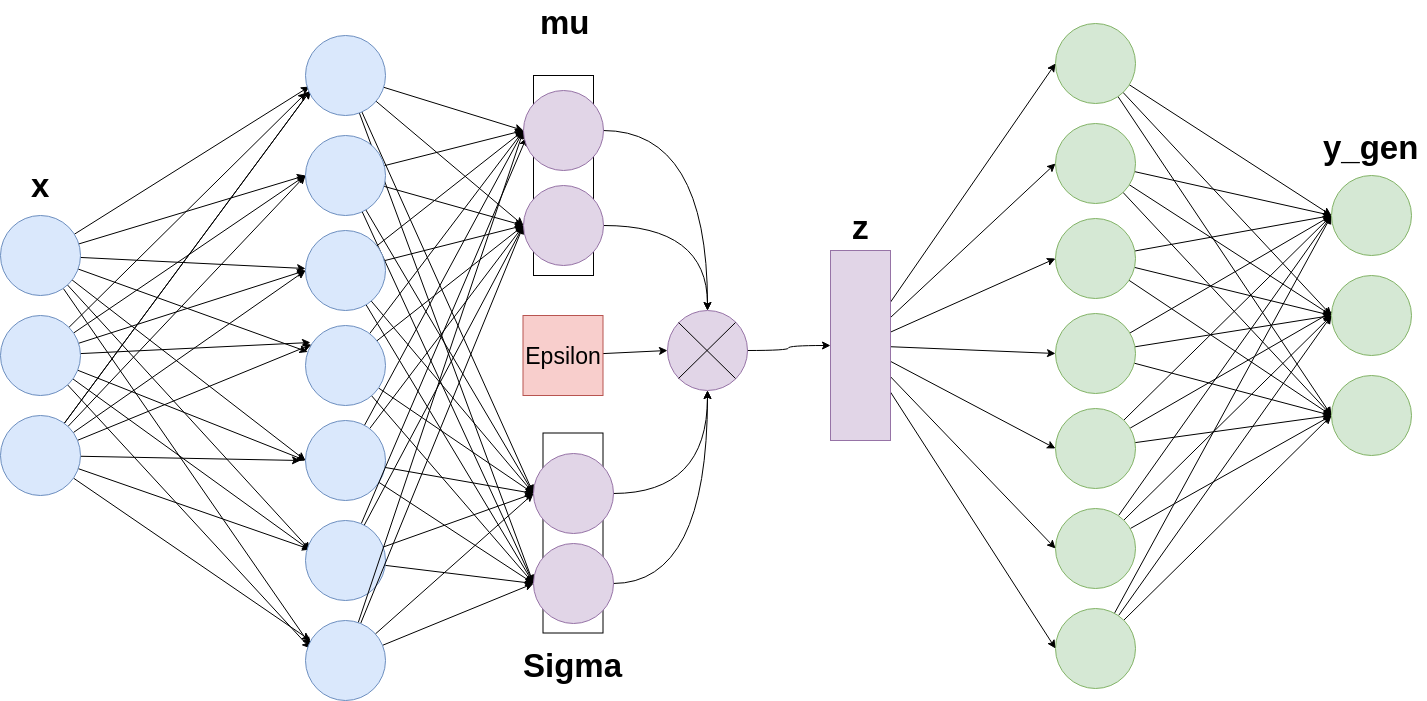
\includegraphics[width=1.0\textwidth]{model}
  \caption{Our implementation, lower amount of neurons displayed}
\end{figure}

It is really close to a default implementation of some VAE. For us, the hidden
layers (so the one between x and $\sigma$, $\mu$) had to be bigger than the x
dimensions, and we used 4x the dimension of x in out code. The mu and the sigma
are the reparametrisation trick from the article, where in order to avoid
sampling but still have some noise in the latent variable z, we use the
following approximation:

$$z = \mu + \sigma \times \epsilon$$

Where epsilon is some random noise.

Then in order to train the model, we needed to have some loss, if we recall the
one used in VAEs:

\begin{align}\label{loss1}
  loss =-D_{KL}\left(
  q_\phi(z|x)||p_\theta(z) \right)+\mathbb{E}_{q_\phi(z|x)}\left[ \log p_\theta(x|z) \right]
\end{align}

We can notice that it is in two parts, the $D_{KL}$ one, which measures how the
encoding distribution of $z$ is similar to the real one, and the reconstruction
loss, so how likely are our generated images knowing the distribution of z,
which is generated by our encoder. For the first part of it, we applied the loss
described in appendix B of the article, where they assume that the prior distribution
of z is a standard gaussian ($N(0, I)$), and where our estimated distribution of
$z$ knowing x is a gaussian ($N(\mu, \sigma)$). We then get an estimation for
$D_{KL}$ using those settings as

\begin{align}\label{loss1}
  -D_{KL}\left(q_\phi(z|x)||p_\theta(z) \right) = \frac{1}{2} \sum\limits_{j=1}^J (1 + log(\sigma_j^2) - \mu^2 - \sigma^2)
\end{align}

For the reconstruction loss, we can just apply some known loss function to know
how good is our model performing. We tried a few, and were quite surprised
sometimes, since the MSE loss for example is performing really badly and we get
almost all the time the same image. The one we finally used is the BCE\_loss,
since we have normalized images, with pixel values normalized, since it's the
one that is performing the better, even if we were also surprised at first.

Finally, the last setting that we found important in order to get good results,
is to use the sum over all individual batch element's loss, and not the mean
over all individual batch element's loss, since this was improving the results a
lot.

This allowed us to get those results, as an example, for the reconstructions we
got from when feeding some images to our model\ref{fig:vae}:

\begin{figure}%
  \centering
  \subfloat[]{{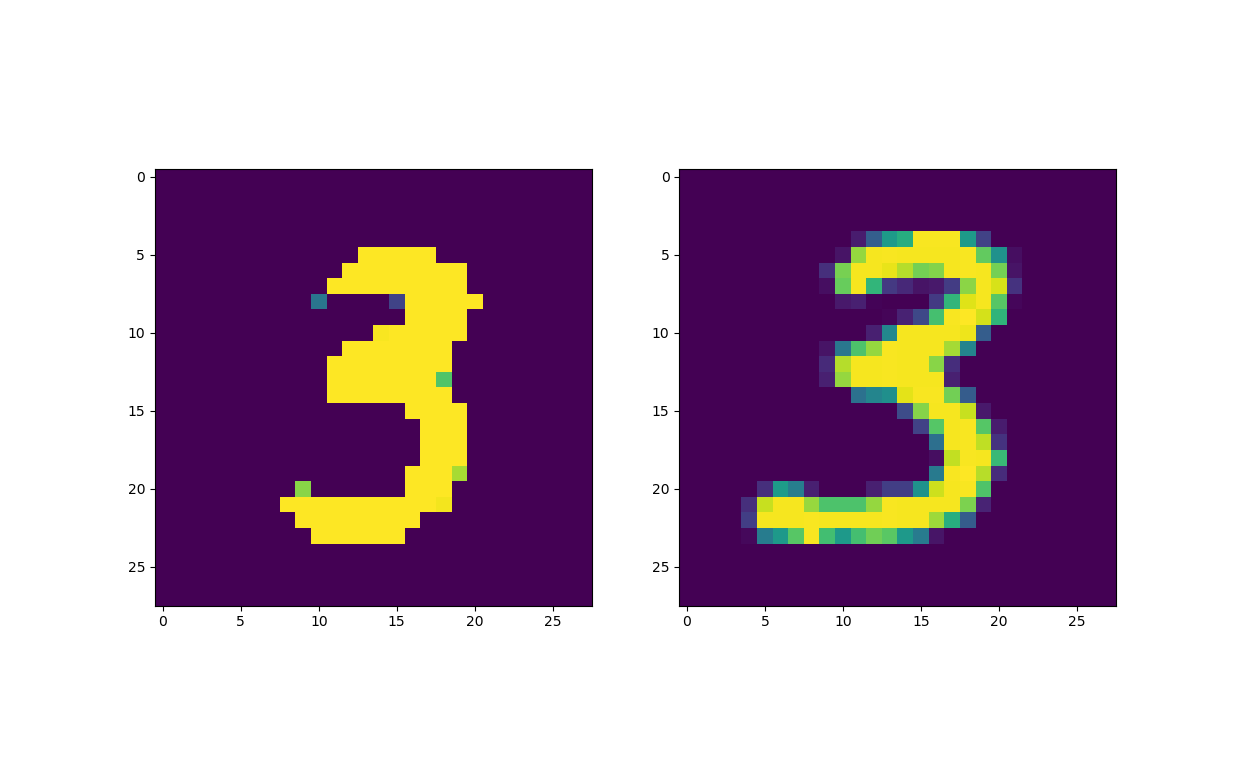
\includegraphics[width=5cm]{VAE_reconstruction_3} }}%
  \qquad
  \subfloat[]{{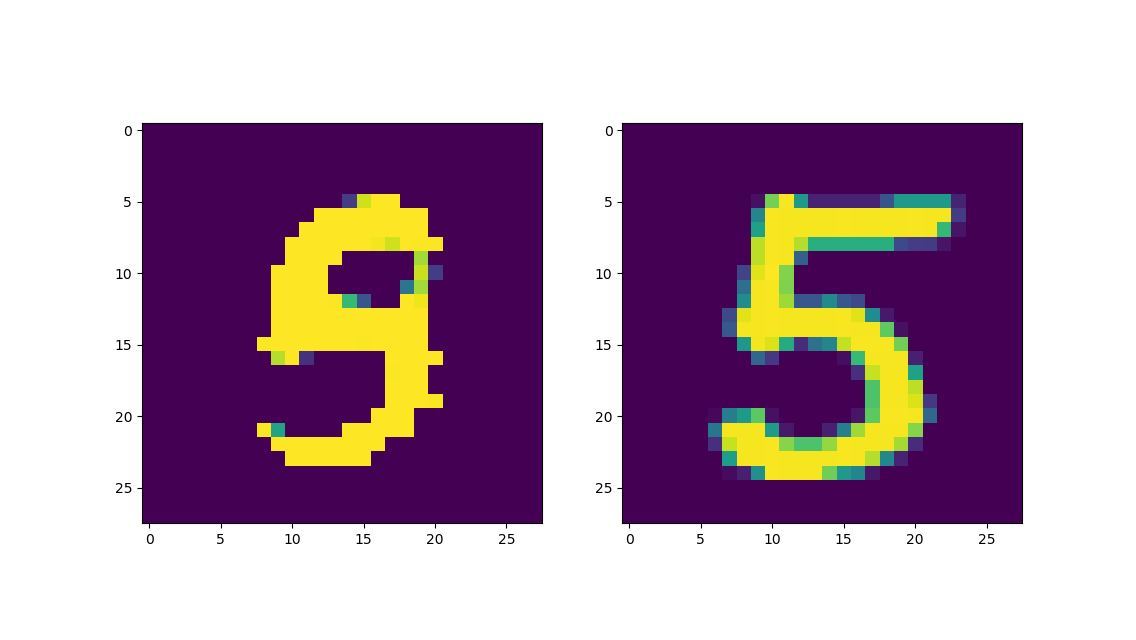
\includegraphics[width=5cm]{VAE_reconstruction_5} }}%
  \caption{Left: VAE reconstruction, right: original MNIST image}%
  \label{fig:vae}%
\end{figure}

For the remaining of the samples showed, they are always taken from the test
set, ie we trained the model on some train set, then, we getting the results or
computing the metric on the results, it was always done on the test set.

Then, let's move forward to the MAE implementation, the goal of this project.   

The MAE version of an autoencoder is really similar to the VAE one, they just
change the loss function to a better performing one. The added two terms to the
VAE loss, one encouraging the diversity of the learned model, the full
explanation of why is not given here but in the article they start from a
measure of diversity, and introduce those two losses that are in practice a
better approximation of the diversity (expecially, they have less variance). The
two added losses are then:

\begin{align}\label{loss1}
  L_{diverse} = E_{X_1, X_2 \sim P(X)}[\sum\limits_{k=1}^Klog(1 + exp(-KL(q_\phi(Z_k|X_1)||q_{\phi}(Z_k|X_2))))]
\end{align}

Where here $\phi$ is still the distribution of the encoder's parameters. This
encourages the diversity of the parameters, since $L_{diverse} \geq 0$ and
$\L_{diverse} \rightarrow 0 \Leftrightarrow
KL(q_\phi(Z_k|X_1)||q_{\phi}(Z_k|X_2)) \rightarrow \infty$, and if this happen
the two distributins are indeed really different depending on the input
datapoint. Here $Z = (Z_1,...,Z_K)$ and hence $Z_k$ is only one element in the
latent variable, not taking this into account make the model behaves really
badly.

The other loss term measures the smoothness of the latent distribution, since
you ideally want them uniformly distributed over the latent space, for ease of
use of the model, and fine grained generation. It is given as:

\begin{align}\label{loss1}
  L_{smooth} = STD_{X_1, X_2 \sim P(X)}[KL(q_\phi(Z_k|X_1)||q_{\phi}(Z_k|X_2))]
\end{align}

And here if the standard deviation is small, then the datapoints are more
uniformly distributed (this comes from the fact that std is not a linear
function, and can be seen in fig1 of MAE article).

We now have the following loss to minimize:

\begin{align}\label{loss1}
  L_{MAE} = L_{ELBO} + \eta L_{diverse} + \gamma L_{smooth}
\end{align}

But how are $L_{diverse}\ and\ L_{smooth}$ computed in practice? Just by using a
monte carlo estimate over the batch, ie using the following formulas, for
example for $L_{diverse}$:

\begin{align}\label{loss1}
  L_{diverse} = \frac{1}{M}\sum\limits_{x_1 \neq x_2}\sum\limits_{k=1}^Klog(1 + exp(-KL(q_\phi(Z_k|X_1)||q_{\phi}(Z_k|X_2))))
\end{align}

Where M is the batch size.

And the KL divergence term is derived from the following formula, assuming
$q_\phi(Z_k|X_1)$ and $q_{\phi}(Z_k|X_2)$ follows normal distribution with there
respective $mu$ and $\sigma$\footnote{href{https://en.wikipedia.org/wiki/Kullback–Leibler\_divergence\#cite\_note-12}{Wikipedia}} :

\begin{align}\label{loss1}
  D_{KL}(N_0||N_1) = \frac{1}{2}(tr(\Sigma_1^{-1}\Sigma_0) + (\mu_1 - \mu_0)^T\Sigma_1^{-1}(\mu_1 - \mu_0) - k + ln(\frac{\det \Sigma_1}{\det \Sigma_0}))
\end{align}

Which can be simplified in our case since we take the batch elements
independently and hence are in one dimension, and wich can be implemented in
python.

By using the same structure for our neural network as the one previously
described for VAE, and by using $\eta = 1$ and $\gamma = 0.01$ we got the
following samples, for example exploring the latent space in one direction:

\begin{figure}
  \centering
      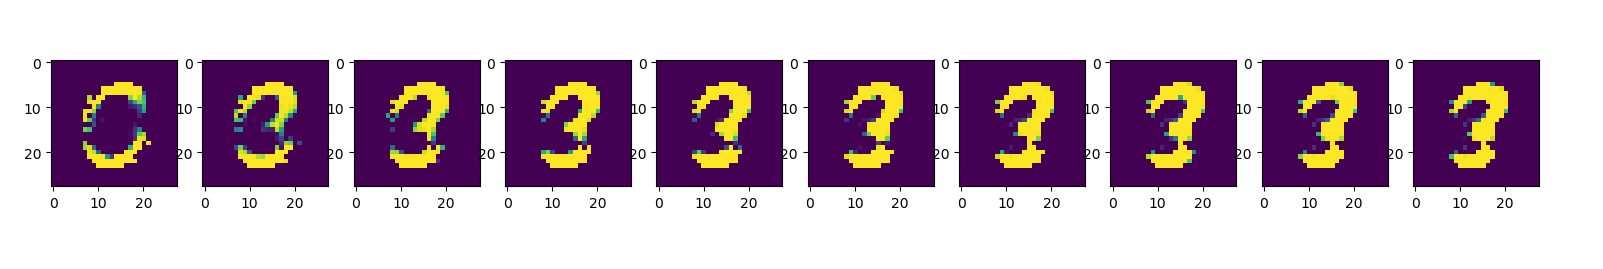
\includegraphics[width=1.0\textwidth]{latent_expl_4}
  \caption{Our implementation, lower amount of neurons displayed}
\end{figure}

Or by testing the reconstruction capabilities of our model:

\begin{figure}%
  \centering
  \subfloat[]{{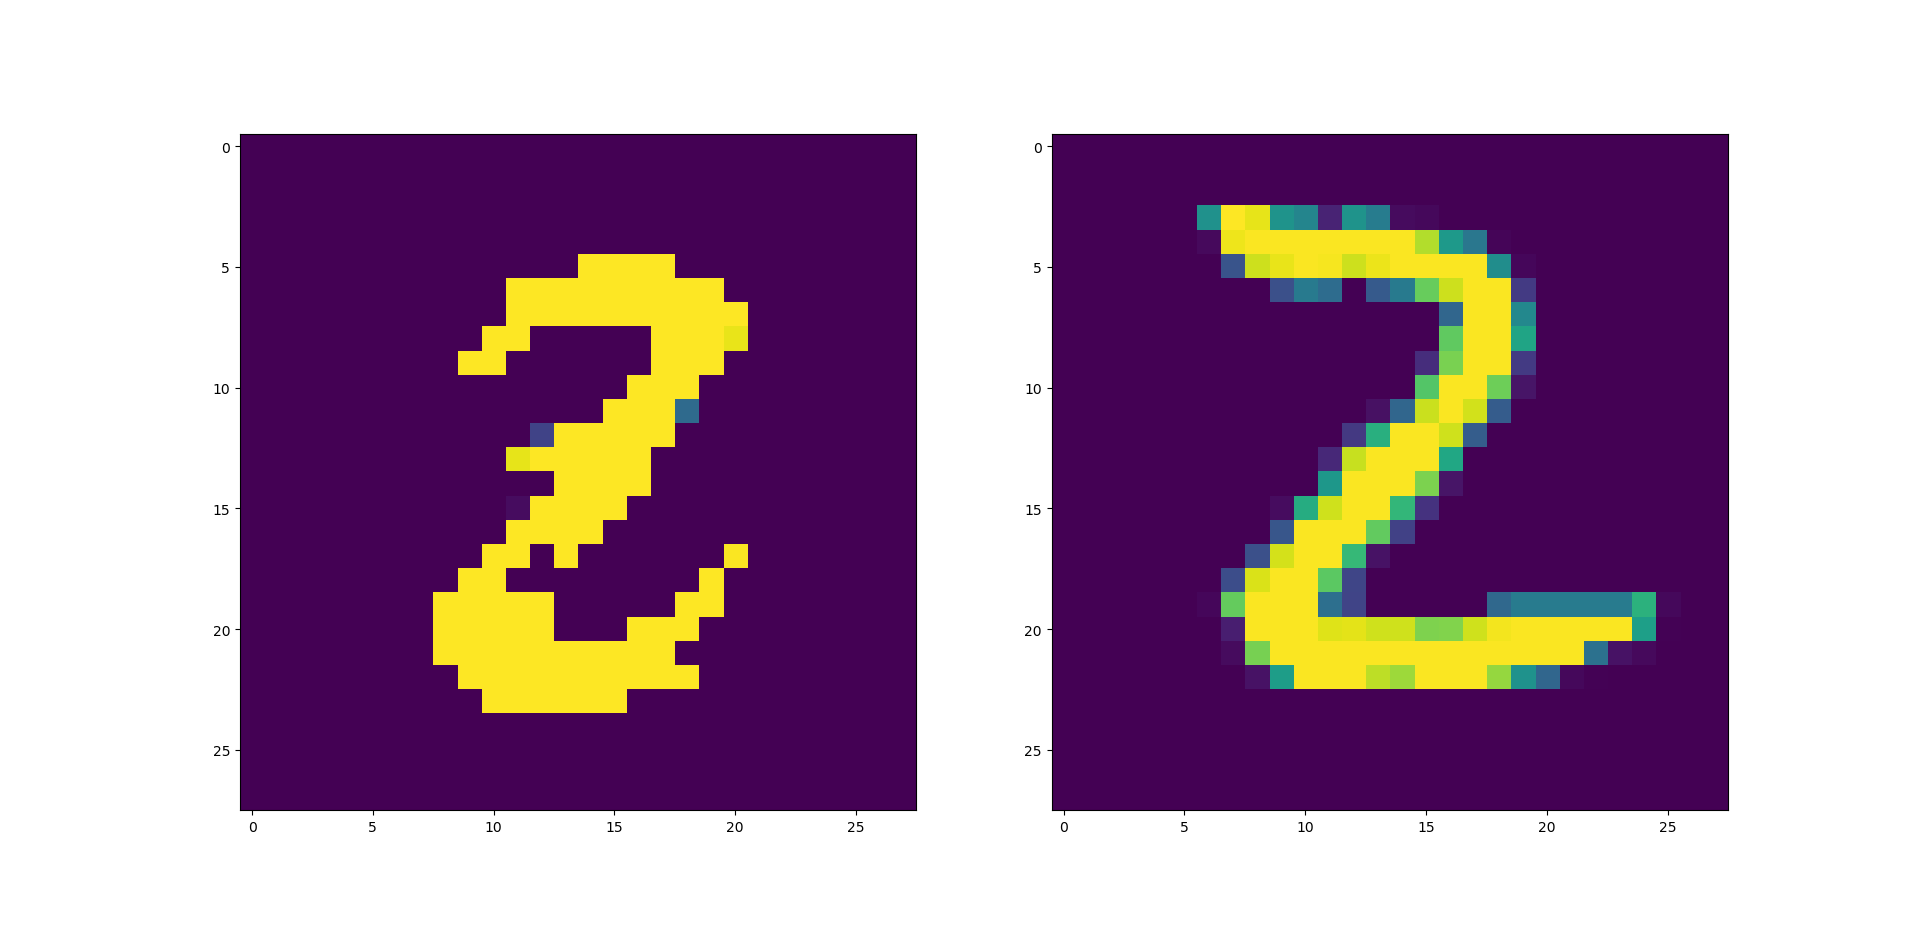
\includegraphics[width=5cm]{reconstruction_22} }}%
  \qquad
  \subfloat[]{{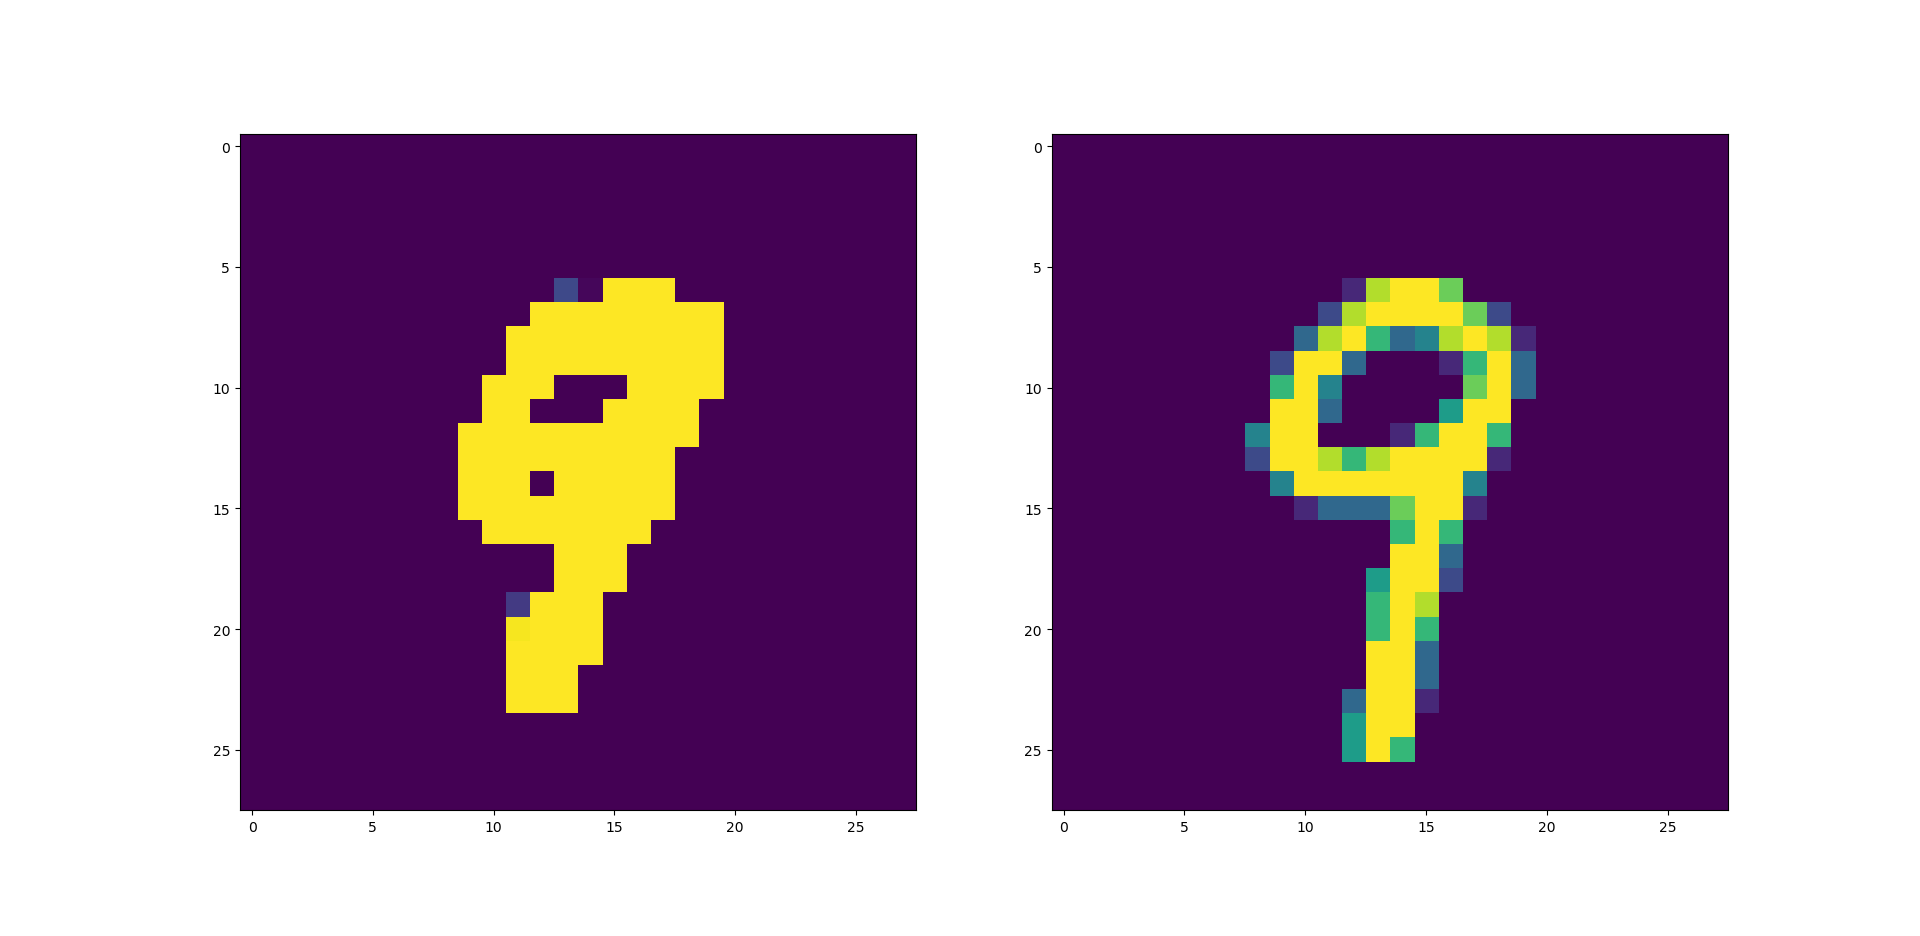
\includegraphics[width=5cm]{reconstruction_99} }}%
  \caption{Left: MAE reconstruction, right: original MNIST image}%
  \label{fig:vae}%
\end{figure}


Finally, we also implemented some convolution based models, for example for the
CIFAR-10 dataset, but they were really long to train, and so we decided to stick
with the MNIST dataset on simple networks.

\subsection{Evaluating our experiments}
Let's now see how we can quantitatively measure how well MAE performs against
the VAE model. Our first attempt to do this was to plot the loss in both cases,
which was indeed smaller in the MAE case, but sincec both of the losses were
negative for some reason, we chose to explore some other direction. We decided
to try to use the K-means algorithm on the latent space, since the MAE results
seemed to be very good in comparison to other models. We implemented the
k-means algorithm, but no matter what we tried, we did not get more than 0.2 for
the accuracy accuracy on the latent variables. Unfortunatelly we didi not had
time to investigate further on this, but it would be some nice future work on
this project.


\section {Conclusion}
Ouverture, future work.
\begin{itemize}
\item extend MAE to other forms of data, in particular text (on which VAEs
  suffer a more serious KL-varnishing problem).
\item Hypespherical Variational Auto-Encoders
  \href{https://arxiv.org/pdf/1804.00891.pdf}{link}. Use another distribution
  than Gaussian to get different latent space (hypespherical structured latent
  space), better suited for some types of data.
\end{itemize}


\nocite{*}
\bibliography{iclr2019_conference}
\bibliographystyle{iclr2019_conference}


\end{document}

